\chapter{Materiali e metodi\ok \ok \ok}

\section{Il Dataset: Severstal steel defect detection \ok}
\begin{comment}

\end{comment}

L'acciaio è uno dei materiali più comunemente utilizzati in tutto il mondo, e la sua produzione è in continua crescita.
La sua versatilità e la sua resistenza lo rendono un materiale molto utilizzato in diversi settori, come l'edilizia, l'automotive, l'industria elettronica, l'industria aerospaziale, ecc.
Per produzioni su larga scala di acciaio come di altri materiali o prodotti, è necessario che il materiale sia di qualità, e che non contenga difetti,
ma è difficile per gli operatori umani rilevare difetti come graffi, crepe, ecc. con elevata affidabilità, per tale ragione 
è necessario adottare sistemi automatizzati che siano in grado di rilevare difetti in modo affidabile e veloce.

L'automatizzazione del controllo qualità è stata la scelta fatta da Severstal, una delle principali aziende produttrici di acciaio in Russia, che produce circa 10 milioni di tonnellate di acciaio 
all'anno. Severstal ha messo a disposizione \"Severstal steel defect detection\" dataset nel 2019 per permettere a chiunque di testarvi le proprie idee, 
sperando di riuscire ad aumentare l'affidabilità del proprio sistema di rilevazione difetti sfruttando la comunita di Kaggle.
Il dataset è disponibile al seguente link: \url{https://www.kaggle.com/c/severstal-steel-defect-detection/data}.

Questo dataset è diviso in 2 parti, training e test set, ma per il test set non sono stati rilasciati i ground truth, quindi non è possibile testare
il modello sul test set originale e verranno dunque utilizzati solo i dati del training set, i quali verranno suddivisi in training e test set.
Il training set originale  è composto da 12568 immagini, che verranno divise in un 50\% per il nuovo training set e 50\% per il nuovo test set, 
quindi un totale di 6284 immagini per il training set e 6284 immagini per il test set. 
Questo numero è stato scelto in modo da garantire un numero minimo di immagini per effettuare l'addestramento del modello, in quanto 
lo scopo non è addestrare un modello perfetto ma valutare l'efficacia del metodo per dataset di piccole dimensioni. 

il training set è stato poi utilizzato per il training del generatore di difetti sintetici, mentre il test set per valutare la qualità dei dati generati
tramite FID score.

\subsection{Distribuzione del dataset}
\begin{comment}
    Cosa posso scrivere in questa sezione?
    - descrizione del dataset
    - descrizione delle immagini
    - descrizione delle classi
    - descrizione della distribuzione delle classi
\end{comment}
In questa sezione viene presentata un'analisi tecnica della distribuzione del dataset, considerando il numero di immagini,
numero e distribuzione dei poligoni in esse, per comprendere nel dettaglio il dataset e la sua composizione.

Il Severstal dataset è composto come già detto da 12568 immagini di lastre di acciaio con risoluzione 1600x256,
di queste immagini abbiamo 6666 immagini con difetti, e 5902 immagini senza difetti. Il severstal dataset presenta 4 classi di difetti,
le quali purtroppo, come spesso accade nei dataset provenienti da casi reali, non sono bilanciate, infatti abbiamo:
\begin{itemize}
    \item poligoni appartenenti alla classe 1 : 3082 
    \item poligoni appartenenti alla classe 2 : 321
    \item poligoni appartenenti alla classe 3 : 14622
    \item poligoni appartenenti alla classe 4 : 1902
\end{itemize}

    \begin{figure}[H]
        \centering
        \begin{tabular}{cc}
            % first row
            \subfloat[Distribuzione delle immagini con e senza difetti.]{
                \label{fig:sd_images_distribution}
                \centering
                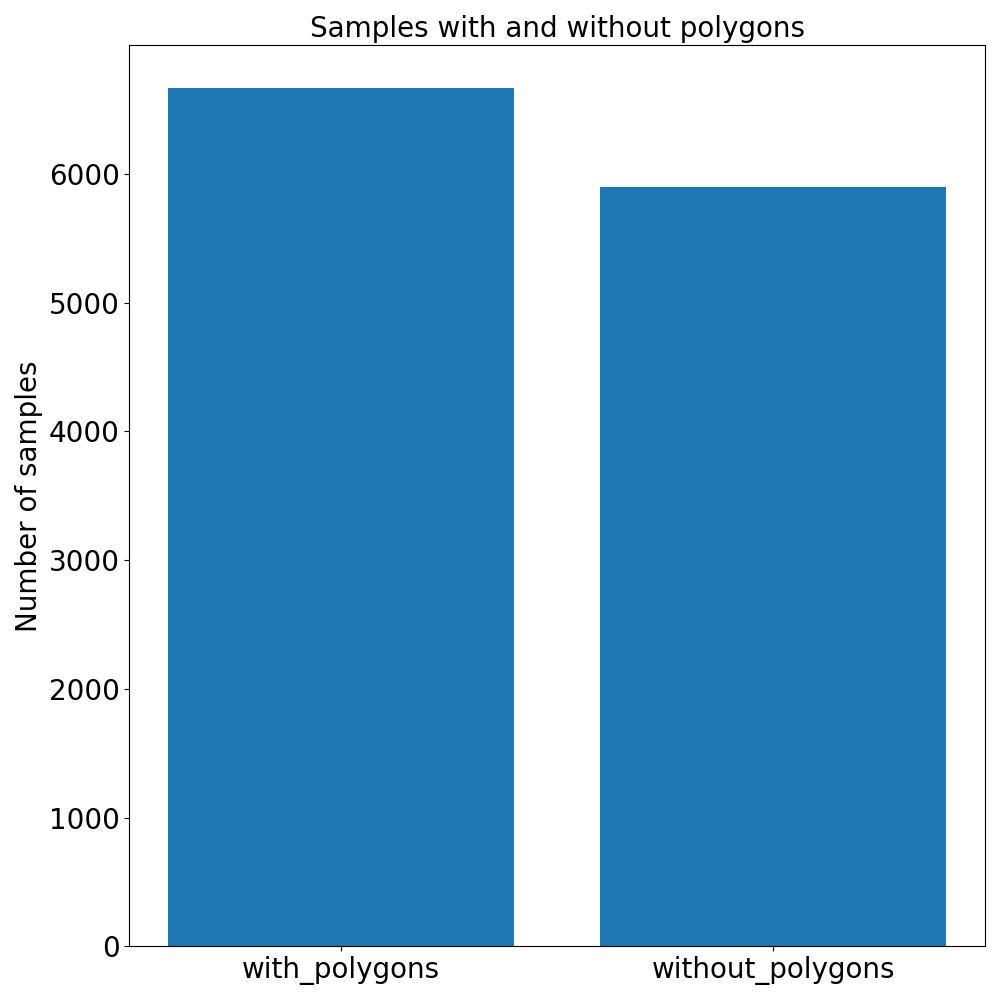
\includegraphics[width=0.45\textwidth]{imgs/Severstal/raw_dataset/samples_with_and_without_polygons_histogram.png}
            }  &
            \subfloat[Distribuzione dei poligoni per classe.]{
                \label{fig:sd_polygons_distribution}
                \centering
                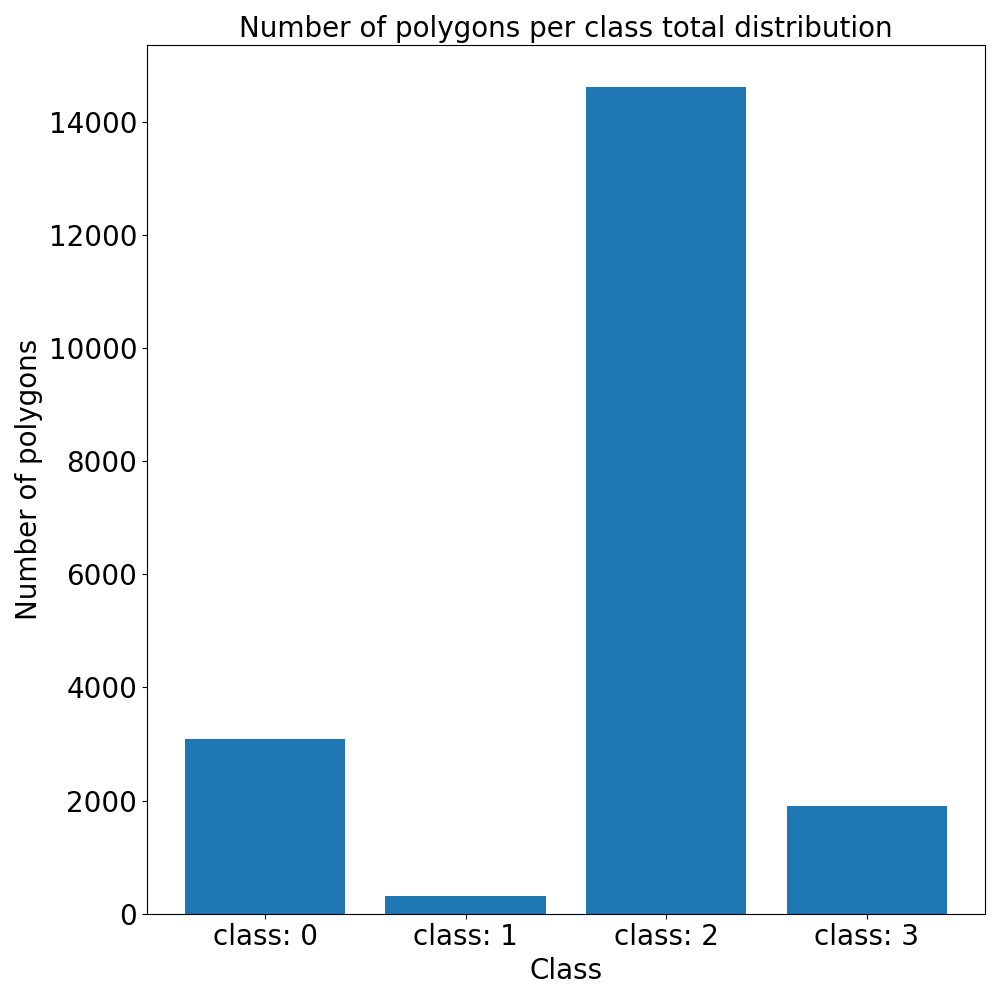
\includegraphics[width=0.45\textwidth]{imgs/Severstal/raw_dataset/n_polygons_per_class_total_histogram.png}
            }  \\
        \end{tabular}
    \end{figure}

Altri parametri interessanti che vanno presi in considerazione riguardano la distribuzione dei poligoni nelle immagini, sono il numero di poligoni
per ogni immagine per avere un'idea della distribuzione. Una valutazione è stata fatto anche per l'area di ogni poligono, in quanto ai fini 
della generazione di difetti sintetici è importante conoscere la quantità di pixel relativa ai difetti a disposizione, consideriamo infatti 
che 10 difetti con area di 100 pixel (1000 pixel) portano con se molta meno informazione di 1 difetto con area di 4000 pixel. 
Le stesse valutazioni sono poi state fatte per ogni classe di difetti, in quanto ogni classe ha una sua specifica distribuzione.

    \begin{figure}[H]
        \centering
        \begin{tabular}{cc}
            % first row
            \subfloat[Distribuzione del numero di poligoni per immagine.]{
                \label{fig:sd_polygons_per_image_distribution}
                \centering
                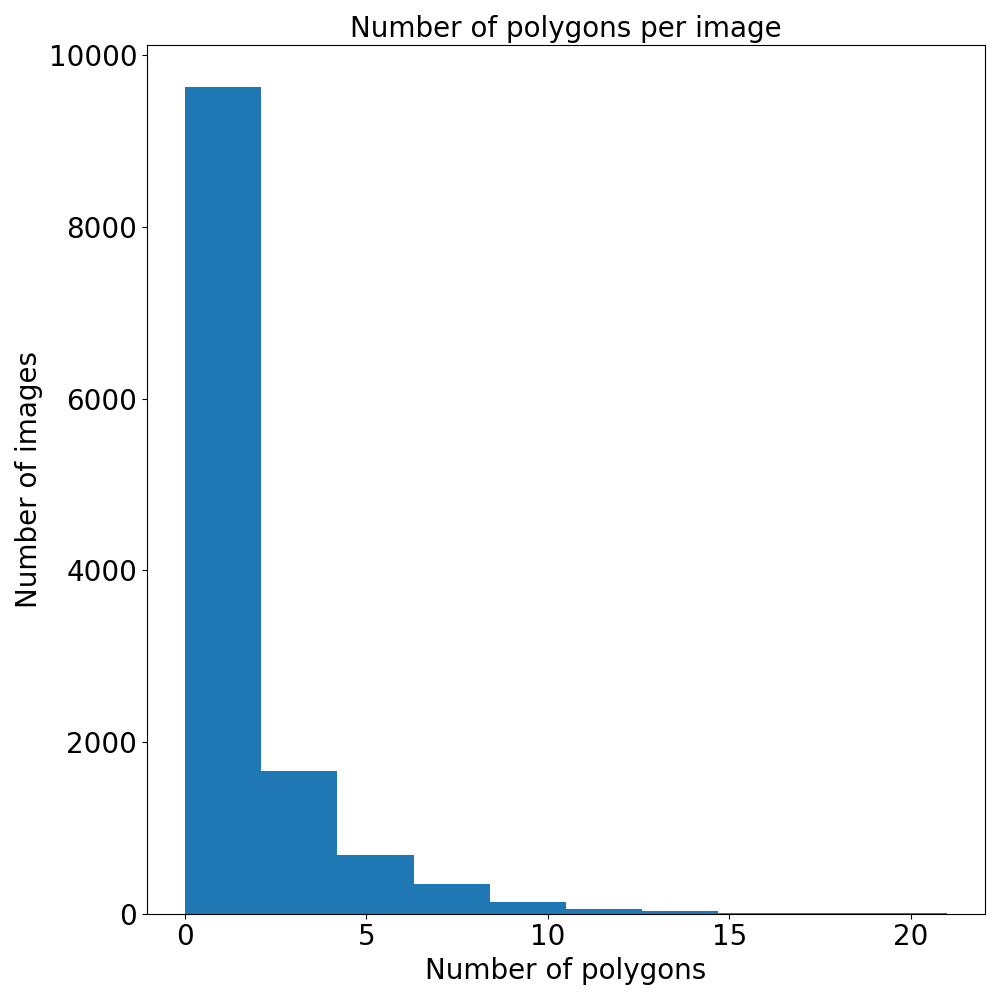
\includegraphics[width=0.45\textwidth]{imgs/Severstal/raw_dataset/n_polygons_per_image_histogram.png}
            }  \\
            \subfloat[Distribuzione del numero di poligoni di classe 1 per immagine]{
                \label{fig:sd_polygons_per_image_per_class_distribution_0}
                \centering
                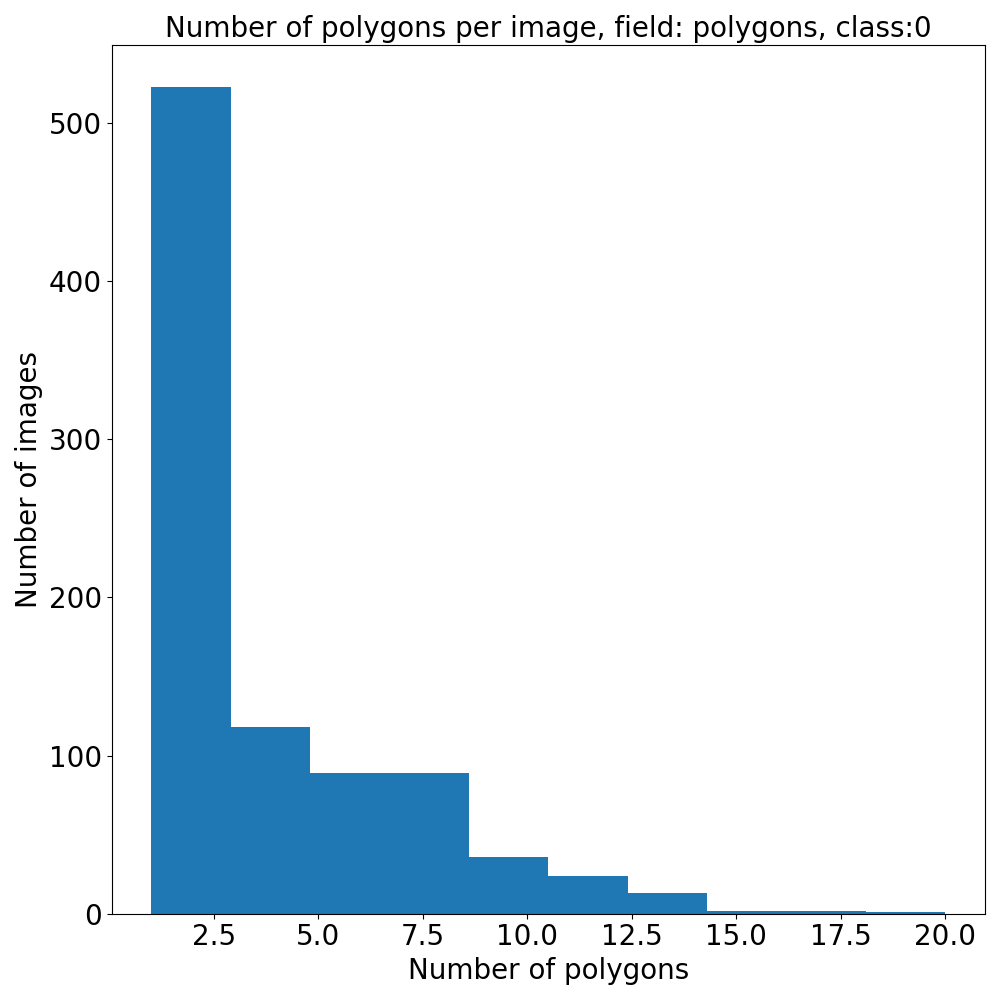
\includegraphics[width=0.45\textwidth]{imgs/Severstal/raw_dataset/n_polygons_per_image_per_class_histogram_polygons_0.png}
            }  &
            \subfloat[Distribuzione del numero di poligoni di classe 2 per immagine]{
                \label{fig:sd_polygons_per_image_per_class_distribution_1}
                \centering
                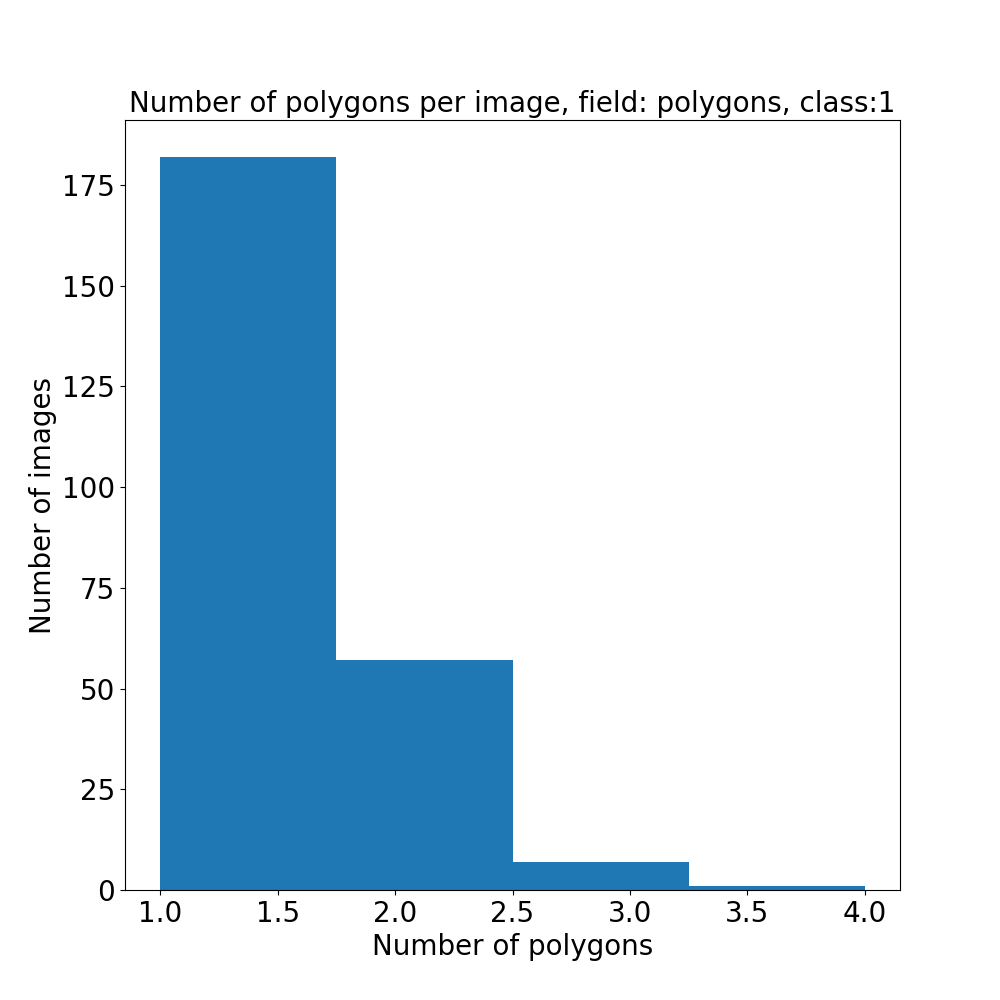
\includegraphics[width=0.45\textwidth]{imgs/Severstal/raw_dataset/n_polygons_per_image_per_class_histogram_polygons_1.png}
            }  \\
            \subfloat[Distribuzione del numero di poligoni di classe 3 per immagine]{
                \label{fig:sd_polygons_per_image_per_class_distribution_2}
                \centering
                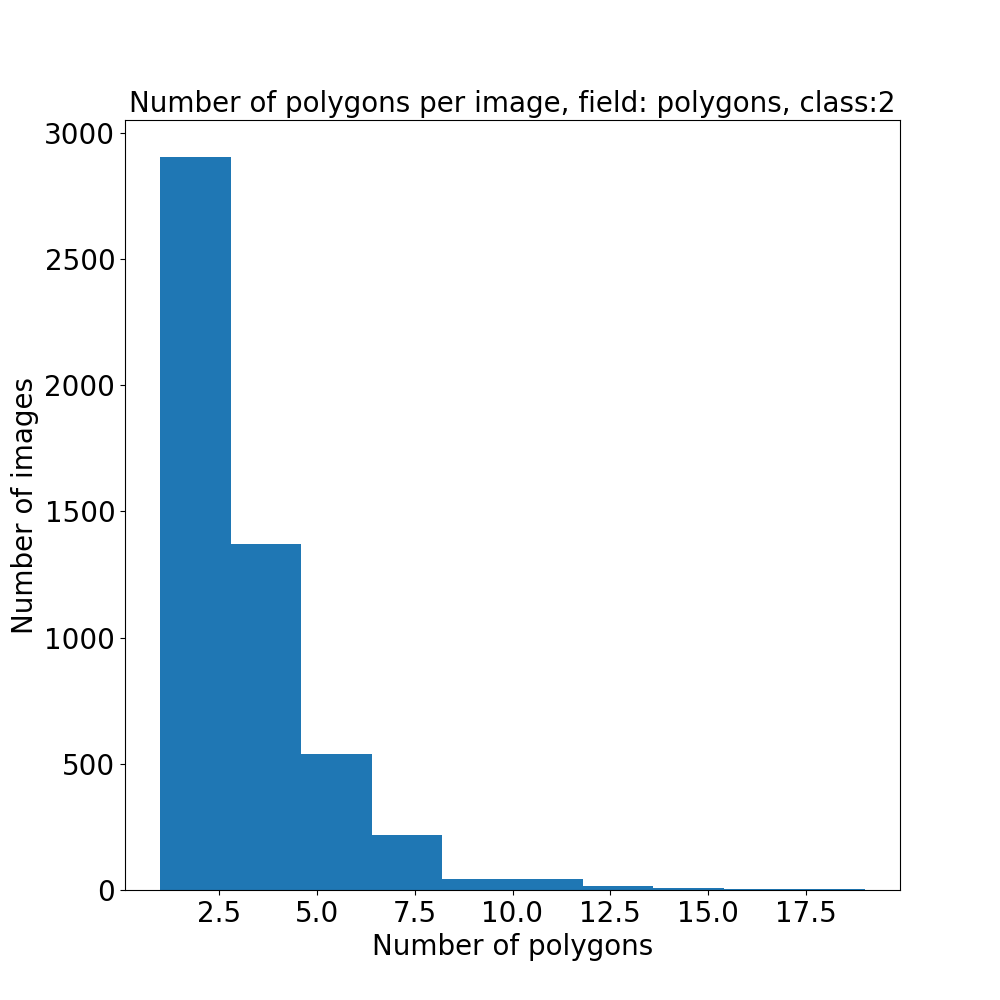
\includegraphics[width=0.45\textwidth]{imgs/Severstal/raw_dataset/n_polygons_per_image_per_class_histogram_polygons_2.png}
            }  &
            \subfloat[Distribuzione del numero di poligoni di classe 4 per immagine]{
                \label{fig:sd_polygons_per_image_per_class_distribution_3}
                \centering
                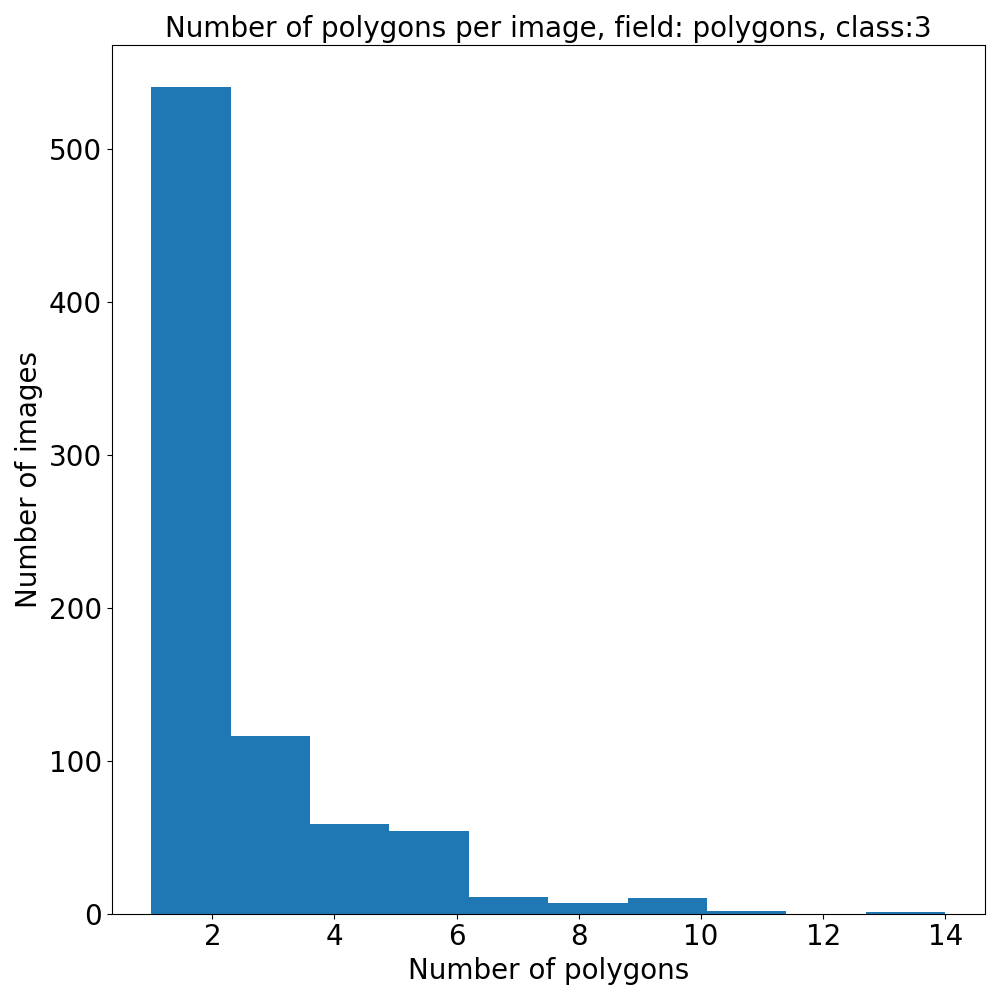
\includegraphics[width=0.45\textwidth]{imgs/Severstal/raw_dataset/n_polygons_per_image_per_class_histogram_polygons_3.png}
            }  \\
        \end{tabular}
    \end{figure}




\section{Librerie e Framework\ok}
\begin{comment}
    In this section i can talk about python and the most important libraries i used
    in the project like pytorch and OpenCv, and why i used them.
\end{comment}
In questo progetto è stato utilizzato il linguaggio python che ad oggi è uno dei linguaggi più utilizzati per il machine learning e l'intelligenza artificiale,
data la sua semplicità e la sua versatilità, per non parlare della vasta scelta di librerie che offre.
Nonostante python sia un linguaggio interpretato, è possibile utilizzarlo per applicazioni che richiedono un alto livello di performance,
in quanto le librerie che si occupano di effettuare le operazioni più pesanti, sono scritte in C/C++, e vengono 
utilizzate tramite python bindings, che permettono di utilizzare le librerie scritte in C/C++ come se fossero state scritte in python,
è questo il caso di librerie come Numpy, OpenCv, Pytorch, ecc.

\subsection{Numpy\ok}
Una delle librerie più importanti per python è Numpy, che permette di lavorare con array multidimensionali, e di effettuare operazioni su di essi 
in modo efficiente con un'interfaccia semplice e intuitiva. Questa libreria benche non sia integrata in python, è una delle librerie più utilizzate
ed è uno standard de facto per il calcolo scientifico per svariate librerie per python.

\subsection{OpenCV\ok}
OpenCV è una libreria open source per il computer vision, scritta in C++, ma utilizzabile anche in python tramite python bindings.
Ad oggi è una delle librerie più utilizzate per l'elaborazione di immagini e video, in quanto offre un'ampia gamma di funzionalità.
In questo progetto è stata utilizzata per effettuare diverse operazioni di pre-elaborazione del dataset, e per lo script demo di inferenza.

\subsection{Pytorch\ok}
Pytorch è una libreria open source per il machine learning, sviluppata da Facebook, che permette di effettuare operazioni su tensori in modo efficiente
sfruttando le GPU, e di effettuare automaticamente il backpropagation, rendendo l'operazione di definire una rete neurale e addestrarla
molto semplice e veloce.
